\subsection{Smooth manifolds}

Let's say we have two intersecting charts: $U_1$ and $U_2$
with maps $\varphi_1$ and $\varphi_2$.
Each of those charts are mapped onto $\mathbb{R}^n$ by their respective local
coordinate maps.
If we consider $U_1 \cap U_2$, we can consider how it's mapped onto $\mathbb{R}^n$
by $\varphi_1$ and $\varphi_2$:

\begin{figure*}[h]
    \centering
    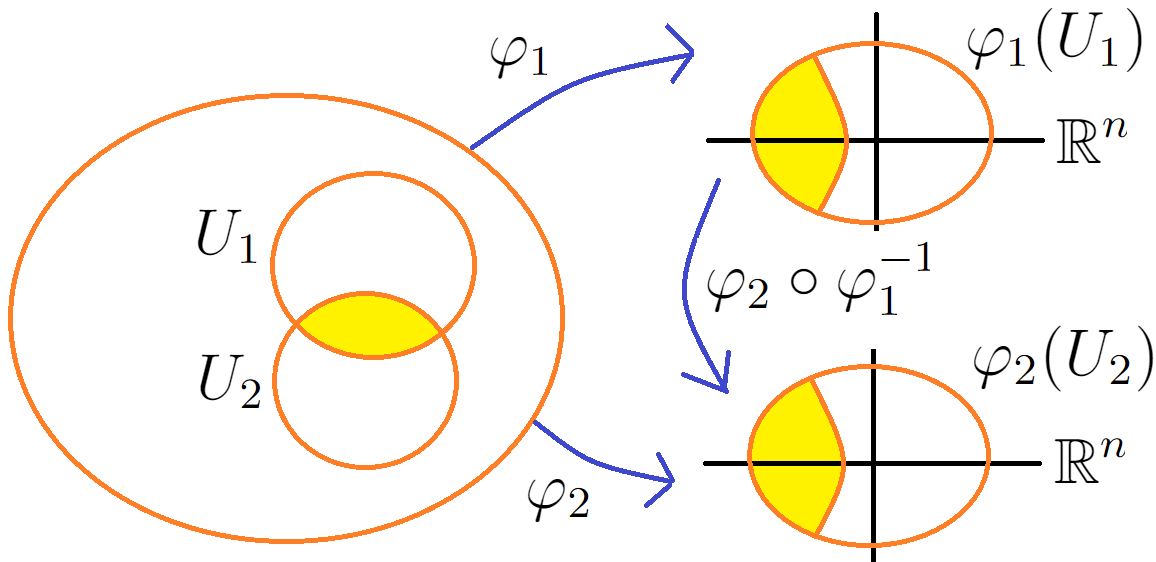
\includegraphics[width=0.7\textwidth]{charts}
\end{figure*}

Since $\varphi_1$ and $\varphi_2$ are both homeomorphisms,
$\varphi_2 \circ \varphi_1^{-1}$ is also a homeomorphism. It will
convert the coordinates of $U_1 \cap U_2$ in the first and in the second chart.

\begin{samepage}
\begin{definition}
    Let $M$ be a topological manifold. 
    Let $\mathcal{A} = \{(U_\alpha, \varphi_\alpha)\}_{\alpha \in I}$, such that:
    \begin{enumerate}
        \item {
            $U_\alpha$ are open and cover $M$.
        }
        \item {
            For all $\alpha, \beta$ with $U_\alpha \cap U_\beta \ne \emptyset$,
            the \textit{transition map}
            \[ 
                \varphi_\beta \circ \varphi_\alpha^{-1} :
                \varphi_\alpha(U_\alpha \cap U_\beta) \to \varphi_\beta(U_\alpha \cap U_\beta)
            \]
            is $C^r$-smooth (i.e., it has $r$ continuous derivatives).
        }
    \end{enumerate}
    Then $\mathcal{A}$ is called a \textit{$C^r$-atlas} of M,
    and the pair $(M, \mathcal{A})$ is called a \textit{$C^r$-manifold}.
\end{definition}
\end{samepage}
\begin{remark}
    This definition is different from the definition of a topological manifold,
    in that now we care about how we glue the charts together --- we want
    it to be smooth.
    If we were to talk about smooth functions on a manifold, then 
    we would run the computations separately on each chart. But in order for 
    those computations to agree with each other, we would need the transition
    functions to be smooth as well.
\end{remark}
\begin{remark}
    By \textit{smooth}  we will mean $C^\infty$-smooth.
\end{remark}

\begin{definition}
    A \textit{$C^r$-differentiable structure} on $M$ is a maximal $C^r$-atlas on
    $\mathcal{A}$ (i.e., not contained in any other $C^r$-atlas).
\end{definition}
\begin{definition}
    Two $C^r$-atlases $\mathcal{A}_1$ and $\mathcal{A}_2$ are \textit{$C^r$-equivalent}, 
    if $\mathcal{A}_1 \cup \mathcal{A}_2$ is a $C^r$-atlas.
\end{definition}
\begin{proposition}
    $C^r$-equivalence is an equivalence relation.
\end{proposition}
\begin{lemma}
    The union of all $C^r$-equivalent atlases in a single equivalence class is
    a maximal atlas. Hence, a maximal atlas exists.
\end{lemma}
\begin{remark}
    We leave the proofs as an exercise.
\end{remark}

There are atlases that don't admit a smooth structure!
For $n = 1, 2, 3, 5, 6$, the $n$-dimensional sphere has only one
smooth structure (i.e. $C^\infty$-differentiable structure).
If $n = 7$ --- there are 28.

Examples of smooth manifolds:
\begin{enumerate}
    \item {
        $\mathbb{R}^n$ --- it has a single chart.
    }
    \item {
        Any open subset of a smooth manifold is a smooth manifold
        (we can intersect the charts with our subset).
    }
    \item {
        A graph of a smooth function $f : \mathbb{R}^n \to \mathbb{R}$.
    }
    \item {
        A sphere $S^n$. We can obtain at least one smooth structure
        using two stereographic projections (as before). The exercise is to check that
        the resulting conversion between those two charts is smooth.
    }
    \item {
        A real projective space $\mathbb{P}^n$. 
        We have defined $\mathbb{P}^n$ before as
        $(x_0, x_1, \dots, x_n) / \sim$ with $n + 1$ different charts,
        depending on which coordinate of a given vector is non-zero.
    }
\end{enumerate}

\begin{remark}
    The smooth structure does not define distances on the manifold.
\end{remark}

\pagebreak
\subsection{Smooth maps between manifolds}
TODO: insert picture.

\begin{definition}
    Let $M$, $N$ be smooth manifolds.
    A map $f : M \to N$ is \textit{smooth} at $p \in M$,
    if there exist charts $(U, \varphi)$ with $p \in U$ and
    $(V, \psi)$ with $f(p) \in V$, such that $f(U) \subset V$ and
    $\psi \circ f \circ \phi^{-1} : \varphi(U) \to \psi(V)$
    is smooth (i.e. infinitely many times differentiable) at $\varphi(p)$.
\end{definition}
\begin{remark}
    The key idea is that if we forget about the maps to $\mathbb{R}^m$/$\mathbb{R}^n$
    and focus solely on $M$ and $N$ themselves, then we simply won't have enough
    structure to define the smoothness of a function.
\end{remark}
\begin{definition}
    $f : M \to N$ is smooth, if it is smooth at every point of $M$.
\end{definition}
\begin{remark}
    If $U \subset \mathbb{R}^m$, then $f : U \to \mathbb{R}^n$
    is smooth if all partial derivatives exist.
\end{remark}
\begin{lemma}
    \label{lem:independentOfChartChoice}
    Smoothness of $f : M \to N$ is independent of the choice of 
    charts in the definition, as long as $f(U) \subset V$.
\end{lemma}
\begin{proof}
    We'll only give the proof idea.
    If we choose other charts, we'll get different $\psi$ and $\phi$ in 
    $\psi \circ f \circ \phi^{-1}$. In order to go back to the original
    $\psi$ and $\phi$, we'll have to compose with the transition maps,
    which are smooth because $M$ and $N$ are smooth manifolds,
    therefore the smoothness is preserved.
\end{proof}
\begin{proposition}
    If $M$, $N$ are smooth manifolds and
    $f : M \to N$ is smooth, then $f$ is continuous (i.e. the preimage of 
    an open set is open),
\end{proposition}
\begin{proof}
    Let's prove it for any point $p \in M$.
    Let's suppose again that $p$ is part of the chart $(U, \varphi)$,
    and $f(p)$ is part of the chart $(V, \psi)$.
    Then we can represent $f|_U$ as
    \[
        f|_U = \varphi^{-1} \circ (\psi \circ f \circ \varphi^{-1}) \circ \varphi
    \]
    $\varphi^{-1}$ is continuous, as it is a homeomorphism. So is $\varphi$.
    $\psi \circ f \circ \varphi^{-1}$ is also continuous, because it is
    smooth in the sense of calculus (i.e. it's a map from $\mathbb{R}^m$ to $\mathbb{R}^n$).
    Therefore, $f|_U$ is continuous as a composition of three continuous functions.

    Therefore, $f$ is continuous at any point $p \in M$, which means that
    $f$ is continuous.
\end{proof}
\begin{proposition}
    \label{prop:propTwoIdk}
    \begin{enumerate}
        \item {
            If $f : M \to N$ and $g : N \to P$ are smooth, then 
            $g \circ f : M \to P$ is smooth.
        }
        \item {
            If $f, g : M \to \mathbb{R}^n$, $\lambda : M \to \mathbb{R}$
            are smooth, then $f + g$, $\lambda g$ and
            $\langle f, g \rangle = \sum f_i(g) \cdot g_i(x)$ are
            smooth functions.
        }
    \end{enumerate}
\end{proposition}
\begin{proof}
    This can be done by the direct application of the definition.
\end{proof}
\begin{definition}[Diffeomorphism]
    Let $M$, $N$  be smooth manifolds. A bijection $f : M \to N$,
    such that $f$ and $f^{-1}$ are smooth is called a 
    \textit{diffeomorphism}.
\end{definition}
\begin{example}
    It can be proved that all compact connected manifolds of dimension 1
    in $\mathbb{R}^2$ are diffeomorphic to a circle.
\end{example}

\subsection{Tangent spaces}
\subsubsection*{Model case}
$M \subset \mathbb{R}^{n+1}$ is a surface given by the graph
of a smooth map $F : \mathbb{R}^n \to \mathbb{R}$.
\[ 
    F(\vec{x} + \vec{v}) = F(\vec{x}) + \nabla F(\vec{x}) \cdot \vec{v} + 
    \textcolor{red}{\vec{o}(\norm{\vec{v}})}
\]
The first two terms are the linear part. They define the tangent space at the point $(\vec{x}, F(\vec{x}))$.
\[
    \nabla F =\Bigl( \frac{\partial F}{\partial x_1}, \dots, 
    \frac{\partial F}{\partial x_n} \Bigr)
    \qquad
    \nabla F(\vec{x}) \vec{v} = \frac{d}{dt} F(\vec{x} + t\vec{v})\Big|_{t=0} =
    D_{\vec{v}} F(\vec{x})
\]
\subsubsection*{General case}
Observe that for $f, g : \mathbb{R}^n \to \mathbb{R}$:
\[ 
    D_{\vec{v}} (fg)(x) = f(x) D_{\vec{v}}(g)(x) + 
    g(x) D_{\vec{v}}(f)(x) 
\]
\begin{definition}
    Let $M$ be a smooth manifold. 
    Let $C^\infty(M)$ denote the space of all $C^\infty$-smooth maps 
    $f: M \to \mathbb{R}$.
\end{definition}
\begin{remark}
    $C^\infty(M)$ is a vector space (by Proposition~\ref{prop:propTwoIdk}),
    and it is not dependent on the choice of charts
    (by Lemma~\ref{lem:independentOfChartChoice}).
\end{remark}
\begin{definition}[Tangent space]
    If $p \in M$, a linear map $D : C^\infty(M) \to \mathbb{R}$ is called a
    \textit{derivation at $p$} if 
    \[ D(fg) = f(p) D(g) + g(p) D(F) \]
    for any $f, g \in C^\infty(M)$.
    Then $T_p M \coloneqq \{D : D \text{ is a derivation at } p \}$
    is called the \textit{tangent space} to $M$ at $p$.
\end{definition}
\begin{lemma}
    Every derivation on $C^\infty(M \subset \mathbb{R}^n)$ at $p$ is some directional
    derivative evaluated at $p$.
\end{lemma}